\documentclass[journal]{IEEEtran}
%\documentclass[technote]{IEEEtran}
\usepackage{ifpdf}
\usepackage{cite}

% vim: nospell
\documentclass[twoside,10pt]{report}

%   Packages
\usepackage[utf8]{inputenc}
\usepackage[T1]{fontenc}
\usepackage[english]{babel}
\usepackage[final]{pdfpages}
\usepackage[section]{placeins}
\usepackage[per-mode = symbol,detect-all=true]{siunitx}
\usepackage[draft,silent,nomargin,inline]{fixme}
\usepackage[compact,noindentafter]{titlesec}
\usepackage{subcaption}
% \usepackage[font{sf,md,up}]{subfig}
% \usepackage[font={small,sf}]{caption}
% \usepackage[scaled=0.83]{helvet}
\usepackage{mathptmx}
\usepackage{courier}
\usepackage{amsmath}
\usepackage{amsfonts}
\usepackage{amssymb}
\usepackage{aurical}
\usepackage{booktabs}
\usepackage{calc}
\usepackage{commath}
\usepackage{pgfplots}
\usepackage{tabularx}
\usepackage{multicol}
\usepackage{graphicx}
\usepackage{gensymb}
\usepackage{url}
\usepackage{tikz}
\usepackage{listings}
\usepackage{hyperref}
\usepackage{longtable}
\usepackage{textcomp}
\usepackage{pdflscape}
\usepackage{float}
\usepackage{lastpage}
\usepackage{xspace}
\usepackage{wasysym}
\usepackage{pageslts}
\usepackage{setspace}
%matlab code font, and such
%   Package setup
\usetikzlibrary{shapes,arrows,positioning,patterns,decorations.markings,decorations.pathmorphing}
\captionsetup[subfigure]{font=normal}
% \usetikzlibrary{external} 
% \tikzexternalize[prefix=img/tikz/]
\tikzset{
    >=latex,
}
\pgfplotsset{
    compat=newest,
    every axis plot/.append style = {
        very thick,
    },
    every axis legend/.append style={
        font={\scriptsize},
    },
    every axis/.append style={
        legend style={draw=none},
        legend cell align=left,
        axis x line=bottom,
        axis y line=left,
        scaled ticks=false,
        xticklabel = \pgfmathparse{\tick*1}\sisetup{scientific-notation = engineering}\num{\pgfmathresult},
        yticklabel = \pgfmathparse{\tick*1}\sisetup{scientific-notation = engineering}\num{\pgfmathresult},
        width=16cm,
        height=5cm,
        axis line style=-latex,
        tick scale binop=\times,
        /pgf/number format/.cd,
        set thousands separator={ },
        set decimal separator={,},
    },
    every axis x label/.style={
        at={(ticklabel* cs:1.00)},
        anchor=west,
    },
    every axis y label/.style={
        at={(ticklabel* cs:1.00)},
        anchor=south,
    },
}
\hypersetup{
    pdfpagelabels=true,
    plainpages=false,
    % pdfauthor={Søren Nørgaard, Miklas Strøm, Jacob Dueholm, Jacob Møller},
    % pdftitle={GFSK Demodulator},
    pdfsubject={},
    bookmarksdepth=3,
    bookmarksnumbered=true,
    colorlinks,
    citecolor=black,
    filecolor=black,
    linkcolor=black,
    urlcolor=black,
    pdfstartview=FitH
}
\usepackage{memhfixc}
\urlstyle{sf}
\sisetup{
    output-decimal-marker = {.},
    output-exponent-marker=\textsc{e}, 
    % round-mode=places,
    output-complex-root=j, 
    % unit-color=blue,
    % scientific-notation = engineering
}
\DeclareSIUnit[number-unit-product = \,]{\permil}{\textperthousand}
\newcolumntype{R}{>{\raggedleft\arraybackslash}X}
\newcolumntype{C}{>{\centering\arraybackslash}X}
\DeclareMathAlphabet{\mathcal}{OMS}{cmsy}{b}{n}

%   Page Setup
\usepackage[top=19mm, bottom=43mm, left=12.925mm, right=12.925mm, a4paper]{geometry}
\setlength{\headheight}{2.5em}  % For fancyhdr
\setlength{\parskip}{0.5em}
\setlength{\parindent}{1.5em}
\renewcommand{\topfraction}{0.85}  % Figures
\renewcommand{\textfraction}{0.1}
\renewcommand{\floatpagefraction}{0.85}
\setcounter{tocdepth}{1}
\setcounter{secnumdepth}{2}

\titlespacing{\chapter}{0em}{0em}{*0}
\titlespacing{\section}{0em}{1em}{*0}
\titlespacing{\subsection}{0pt}{1em}{*0}
\titlespacing{\subsubsection}{0pt}{1em}{*0}
% \titleformat{name=\part}[display] {}{}{0em}{\fontfamily{phv}\fontsize{40}{48}\selectfont\centering\bfseries\thepart\\}
% \titleformat{name=\chapter}[display] {}{}{0em}{\fontfamily{phv}\selectfont\huge\thechapter\ }
% \titleformat{name=\chapter,numberless}[display] {}{}{0em}{\fontfamily{phv}\selectfont\huge}
% \titleformat{name=\section}[display] {}{}{0em}{\fontfamily{phv}\selectfont\bfseries\Large\thesection\ }
% \titleformat{name=\section}[display] {}{}{0em}{\bfseries\Large\thesection\ }
% \titleformat{name=\subsection}[display] {}{}{0em}{\fontfamily{phv}\selectfont\Large\thesubsection\ }
% \titleformat{name=\subsubsection}[display] {}{}{0em}{\normalsize\bfseries}
% \titleformat{name=\paragraph}[runin] {}{}{0em}{\normalsize\itshape}

%   Header and Items
\usepackage{fancyhdr}
\renewcommand{\headrulewidth}{0pt}
\pagestyle{fancy}
\fancyfoot{}{}{}
\fancyhead[LO]{\normalsize\rightmark}
\fancyhead[RE]{\normalsize\leftmark}
\fancyhead[LE,RO]{\normalsize\thepage}
\let\tempone\itemize
\let\temptwo\enditemize
\renewenvironment{itemize}{%
    \tempone%
    \setlength{\parskip}{0em}%
    \setlength{\itemsep}{0.25em}%
    }{\temptwo}
\let\tempthree\enumerate
\let\tempfour\endenumerate
\renewenvironment{enumerate}{%
    \tempthree%
    \setlength{\parskip}{0em}%
    \setlength{\itemsep}{0.25em}%
    }{\tempfour}
\let\tempfive\description
\let\tempsix\enddescription
\renewenvironment{description}{%
    \tempfive%
    \setlength{\parskip}{0em}%
    \setlength{\itemsep}{0.25em}%
    }{\tempsix}
\renewcommand{\labelenumi}{\arabic{enumi}.}
\renewcommand{\labelenumii}{\arabic{enumi}.~\arabic{enumii}}
\renewcommand{\labelenumiii}{\arabic{enumi}.~\arabic{enumii}.~\arabic{enumiii}}
\graphicspath{{./img/}}

%   Packages (must be loaded last)
\usepackage{csvsimple}
\usepackage[american]{circuitikz}

% \usepackage{set/showlabels,rotating}
% \renewcommand{\showlabelsetlabel}[1]%
% {\begin{turn}{80}\showlabelfont\tiny #1\end{turn}}

% COOL LOOKING FONT!!!
% \usepackage{pdfrender}
% \pdfrender{StrokeColor=black,TextRenderingMode=2,LineWidth=0.2pt}


%
%\ifCLASSINFOpdf
  % \usepackage[pdftex]{graphicx}
  % declare the path(s) where your graphic files are
  % \graphicspath{{../pdf/}{../jpeg/}}
  % and their extensions so you won't have to specify these with
  % every instance of \includegraphics
  % \DeclareGraphicsExtensions{.pdf,.jpeg,.png}
%\else
  % or other class option (dvipsone, dvipdf, if not using dvips). graphicx
  % will default to the driver specified in the system graphics.cfg if no
  % driver is specified.
  % \usepackage[dvips]{graphicx}
  % declare the path(s) where your graphic files are
  % \graphicspath{{../eps/}}
  % and their extensions so you won't have to specify these with
  % every instance of \includegraphics
  % \DeclareGraphicsExtensions{.eps}
%\fi
% graphicx was written by David Carlisle and Sebastian Rahtz. It is
% required if you want graphics, photos, etc. graphicx.sty is already
% installed on most LaTeX systems. The latest version and documentation
% can be obtained at: 
% http://www.ctan.org/pkg/graphicx
% Another good source of documentation is "Using Imported Graphics in
% LaTeX2e" by Keith Reckdahl which can be found at:
% http://www.ctan.org/pkg/epslatex
%
% latex, and pdflatex in dvi mode, support graphics in encapsulated
% postscript (.eps) format. pdflatex in pdf mode supports graphics
% in .pdf, .jpeg, .png and .mps (metapost) formats. Users should ensure
% that all non-photo figures use a vector format (.eps, .pdf, .mps) and
% not a bitmapped formats (.jpeg, .png). The IEEE frowns on bitmapped formats
% which can result in "jaggedy"/blurry rendering of lines and letters as
% well as large increases in file sizes.
%
% You can find documentation about the pdfTeX application at:
% http://www.tug.org/applications/pdftex





% *** MATH PACKAGES ***
%
%\usepackage{amsmath}
% A popular package from the American Mathematical Society that provides
% many useful and powerful commands for dealing with mathematics.
%
% Note that the amsmath package sets \interdisplaylinepenalty to 10000
% thus preventing page breaks from occurring within multiline equations. Use:
%\interdisplaylinepenalty=2500
% after loading amsmath to restore such page breaks as IEEEtran.cls normally
% does. amsmath.sty is already installed on most LaTeX systems. The latest
% version and documentation can be obtained at:
% http://www.ctan.org/pkg/amsmath





% *** SPECIALIZED LIST PACKAGES ***
%
%\usepackage{algorithmic}
% algorithmic.sty was written by Peter Williams and Rogerio Brito.
% This package provides an algorithmic environment fo describing algorithms.
% You can use the algorithmic environment in-text or within a figure
% environment to provide for a floating algorithm. Do NOT use the algorithm
% floating environment provided by algorithm.sty (by the same authors) or
% algorithm2e.sty (by Christophe Fiorio) as the IEEE does not use dedicated
% algorithm float types and packages that provide these will not provide
% correct IEEE style captions. The latest version and documentation of
% algorithmic.sty can be obtained at:
% http://www.ctan.org/pkg/algorithms
% Also of interest may be the (relatively newer and more customizable)
% algorithmicx.sty package by Szasz Janos:
% http://www.ctan.org/pkg/algorithmicx




% *** ALIGNMENT PACKAGES ***
%
%\usepackage{array}
% Frank Mittelbach's and David Carlisle's array.sty patches and improves
% the standard LaTeX2e array and tabular environments to provide better
% appearance and additional user controls. As the default LaTeX2e table
% generation code is lacking to the point of almost being broken with
% respect to the quality of the end results, all users are strongly
% advised to use an enhanced (at the very least that provided by array.sty)
% set of table tools. array.sty is already installed on most systems. The
% latest version and documentation can be obtained at:
% http://www.ctan.org/pkg/array


% IEEEtran contains the IEEEeqnarray family of commands that can be used to
% generate multiline equations as well as matrices, tables, etc., of high
% quality.




% *** SUBFIGURE PACKAGES ***
%\ifCLASSOPTIONcompsoc
%  \usepackage[caption=false,font=normalsize,labelfont=sf,textfont=sf]{subfig}
%\else
%  \usepackage[caption=false,font=footnotesize]{subfig}
%\fi
% subfig.sty, written by Steven Douglas Cochran, is the modern replacement
% for subfigure.sty, the latter of which is no longer maintained and is
% incompatible with some LaTeX packages including fixltx2e. However,
% subfig.sty requires and automatically loads Axel Sommerfeldt's caption.sty
% which will override IEEEtran.cls' handling of captions and this will result
% in non-IEEE style figure/table captions. To prevent this problem, be sure
% and invoke subfig.sty's "caption=false" package option (available since
% subfig.sty version 1.3, 2005/06/28) as this is will preserve IEEEtran.cls
% handling of captions.
% Note that the Computer Society format requires a larger sans serif font
% than the serif footnote size font used in traditional IEEE formatting
% and thus the need to invoke different subfig.sty package options depending
% on whether compsoc mode has been enabled.
%
% The latest version and documentation of subfig.sty can be obtained at:
% http://www.ctan.org/pkg/subfig




% *** FLOAT PACKAGES ***
%
%\usepackage{fixltx2e}
% fixltx2e, the successor to the earlier fix2col.sty, was written by
% Frank Mittelbach and David Carlisle. This package corrects a few problems
% in the LaTeX2e kernel, the most notable of which is that in current
% LaTeX2e releases, the ordering of single and double column floats is not
% guaranteed to be preserved. Thus, an unpatched LaTeX2e can allow a
% single column figure to be placed prior to an earlier double column
% figure.
% Be aware that LaTeX2e kernels dated 2015 and later have fixltx2e.sty's
% corrections already built into the system in which case a warning will
% be issued if an attempt is made to load fixltx2e.sty as it is no longer
% needed.
% The latest version and documentation can be found at:
% http://www.ctan.org/pkg/fixltx2e


%\usepackage{stfloats}
% stfloats.sty was written by Sigitas Tolusis. This package gives LaTeX2e
% the ability to do double column floats at the bottom of the page as well
% as the top. (e.g., "\begin{figure*}[!b]" is not normally possible in
% LaTeX2e). It also provides a command:
%\fnbelowfloat
% to enable the placement of footnotes below bottom floats (the standard
% LaTeX2e kernel puts them above bottom floats). This is an invasive package
% which rewrites many portions of the LaTeX2e float routines. It may not work
% with other packages that modify the LaTeX2e float routines. The latest
% version and documentation can be obtained at:
% http://www.ctan.org/pkg/stfloats
% Do not use the stfloats baselinefloat ability as the IEEE does not allow
% \baselineskip to stretch. Authors submitting work to the IEEE should note
% that the IEEE rarely uses double column equations and that authors should try
% to avoid such use. Do not be tempted to use the cuted.sty or midfloat.sty
% packages (also by Sigitas Tolusis) as the IEEE does not format its papers in
% such ways.
% Do not attempt to use stfloats with fixltx2e as they are incompatible.
% Instead, use Morten Hogholm'a dblfloatfix which combines the features
% of both fixltx2e and stfloats:
%
% \usepackage{dblfloatfix}
% The latest version can be found at:
% http://www.ctan.org/pkg/dblfloatfix




%\ifCLASSOPTIONcaptionsoff
%  \usepackage[nomarkers]{endfloat}
% \let\MYoriglatexcaption\caption
% \renewcommand{\caption}[2][\relax]{\MYoriglatexcaption[#2]{#2}}
%\fi
% endfloat.sty was written by James Darrell McCauley, Jeff Goldberg and 
% Axel Sommerfeldt. This package may be useful when used in conjunction with 
% IEEEtran.cls'  captionsoff option. Some IEEE journals/societies require that
% submissions have lists of figures/tables at the end of the paper and that
% figures/tables without any captions are placed on a page by themselves at
% the end of the document. If needed, the draftcls IEEEtran class option or
% \CLASSINPUTbaselinestretch interface can be used to increase the line
% spacing as well. Be sure and use the nomarkers option of endfloat to
% prevent endfloat from "marking" where the figures would have been placed
% in the text. The two hack lines of code above are a slight modification of
% that suggested by in the endfloat docs (section 8.4.1) to ensure that
% the full captions always appear in the list of figures/tables - even if
% the user used the short optional argument of \caption[]{}.
% IEEE papers do not typically make use of \caption[]'s optional argument,
% so this should not be an issue. A similar trick can be used to disable
% captions of packages such as subfig.sty that lack options to turn off
% the subcaptions:
% For subfig.sty:
% \let\MYorigsubfloat\subfloat
% \renewcommand{\subfloat}[2][\relax]{\MYorigsubfloat[]{#2}}
% However, the above trick will not work if both optional arguments of
% the \subfloat command are used. Furthermore, there needs to be a
% description of each subfigure *somewhere* and endfloat does not add
% subfigure captions to its list of figures. Thus, the best approach is to
% avoid the use of subfigure captions (many IEEE journals avoid them anyway)
% and instead reference/explain all the subfigures within the main caption.
% The latest version of endfloat.sty and its documentation can obtained at:
% http://www.ctan.org/pkg/endfloat
%
% The IEEEtran \ifCLASSOPTIONcaptionsoff conditional can also be used
% later in the document, say, to conditionally put the References on a 
% page by themselves.

% *** PDF, URL AND HYPERLINK PACKAGES ***
%
%\usepackage{url}
% url.sty was written by Donald Arseneau. It provides better support for
% handling and breaking URLs. url.sty is already installed on most LaTeX
% systems. The latest version and documentation can be obtained at:
% http://www.ctan.org/pkg/url
% Basically, \url{my_url_here}.

% *** Do not adjust lengths that control margins, column widths, etc. ***
% *** Do not use packages that alter fonts (such as pslatex).         ***
% There should be no need to do such things with IEEEtran.cls V1.6 and later.
% (Unless specifically asked to do so by the journal or conference you plan
% to submit to, of course. )


% correct bad hyphenation here
% \hyphenation{op-tical net-works semi-conduc-tor}


\begin{document}
%
% paper title
% Titles are generally capitalized except for words such as a, an, and, as,
% at, but, by, for, in, nor, of, on, or, the, to and up, which are usually
% not capitalized unless they are the first or last word of the title.
% Linebreaks \\ can be used within to get better formatting as desired.
% Do not put math or special symbols in the title.
\title{LTE MIMO Antennas With 5\,mm Ground Clearance}
%
%
% author names and IEEE memberships
% note positions of commas and nonbreaking spaces ( ~ ) LaTeX will not break
% a structure at a ~ so this keeps an author's name from being broken across
% two lines.
% use \thanks{} to gain access to the first footnote area
% a separate \thanks must be used for each paragraph as LaTeX2e's \thanks
% was not built to handle multiple paragraphs
%

\author{Lasse Thomsen, Henrik Aarup Vesterager, Søren Bøgeskov Nørgaard}% <-this % stops a space
\thanks{Lasse Thomsen, Henrik Aarup Vesterager, and Søren Bøgeskov Nørgaard are with the Antennas, Propagation and Radio Networking section at the Department of Electronic Systems, Aalborg University, Denmark (email: \{lthom11,have11,snarga11\}@student.aau.dk).}% <-this % stops a space
%\thanks{J. Doe and J. Doe are with Anonymous University.}% <-this % stops a space
%\thanks{Manuscript received April 19, 2005; revised August 26, 2015.}

% note the % following the last \IEEEmembership and also \thanks - 
% these prevent an unwanted space from occurring between the last author name
% and the end of the author line. i.e., if you had this:
% 
% \author{....lastname \thanks{...} \thanks{...} }
%                     ^------------^------------^----Do not want these spaces!
%
% a space would be appended to the last name and could cause every name on that
% line to be shifted left slightly. This is one of those "LaTeX things". For
% instance, "\textbf{A} \textbf{B}" will typeset as "A B" not "AB". To get
% "AB" then you have to do: "\textbf{A}\textbf{B}"
% \thanks is no different in this regard, so shield the last } of each \thanks
% that ends a line with a % and do not let a space in before the next \thanks.
% Spaces after \IEEEmembership other than the last one are OK (and needed) as
% you are supposed to have spaces between the names. For what it is worth,
% this is a minor point as most people would not even notice if the said evil
% space somehow managed to creep in.



% The paper headers
%\markboth{Journal of \LaTeX\ Class Files,~Vol.~14, No.~8, August~2015}%
%{Shell \MakeLowercase{\textit{et al.}}: Bare Demo of IEEEtran.cls for IEEE Journals}
% The only time the second header will appear is for the odd numbered pages
% after the title page when using the twoside option.
% 
% *** Note that you probably will NOT want to include the author's ***
% *** name in the headers of peer review papers.                   ***
% You can use \ifCLASSOPTIONpeerreview for conditional compilation here if
% you desire.


% If you want to put a publisher's ID mark on the page you can do it like
% this:
%\IEEEpubid{0000--0000/00\$00.00~\copyright~2015 IEEE}
% Remember, if you use this you must call \IEEEpubidadjcol in the second
% column for its text to clear the IEEEpubid mark.

% use for special paper notices
%\IEEEspecialpapernotice{(Invited Paper)}

% make the title area
\maketitle
\setcounter{page}{1}
% As a general rule, do not put math, special symbols or citations
% in the abstract or keywords.
\begin{abstract}
% Intro
The internal antennas of today's smartphones are often placed along the edge of the phone due to limited space and strict size requirements. As a result, the antennas are in very close proximity to the user. This results in detuning of the antenna and power absorption by the user. As the demand for higher data rates and bandwidth keeps increasing, it is desirable to counteract the detuning \cite{hilbert2015tradeoff}.    

This project will investigate the development of digitally tunable LTE antennas, with minimized ground clearance, supporting MIMO.
The solution proposes the use of a digitally controllable MEMS tuner in the matching network.


% Three designs
To investigate the tunable performance and the user effect interaction, three prototype designs have been simulated and measured. Three user effect cases have been simulated for each prototype and generally, the antennas shows detuning as an effect of the user interaction. 
The prototype results have been compared and the best performing antenna design has been moved to and measured on a PCB with a WiSpry WS1040 digital tuner for each antenna.

% Ground clearance
A ground clearance investigation has been carried out and it was found, that a decent bandwidth can be obtained with only \SI{5}{mm} of ground clearance. This lead to a new antenna design with \SI{5}{mm} ground clearance, which has been measured on the tuner PCB.

% PCB problems
Moving the two antenna designs from the prototype PCB to the tuner PCB introduces some high band coverage problems. The antenna and the transmission line have been modified to counteract these problems.  

% Conclusion
A MIMO tunable antenna solution has been presented with a minimized ground clearance of \SI{5}{mm}. The results show promising and comparable performance with state-of-the-art antenna designs with much higher ground clearance.

\end{abstract}

% Note that keywords are not normally used for peerreview papers.
\begin{IEEEkeywords}
Mobile terminal antenna, LTE, MIMO, ground clearance
\end{IEEEkeywords}

% For peer review papers, you can put extra information on the cover
% page as needed:
% \ifCLASSOPTIONpeerreview
% \begin{center} \bfseries EDICS Category: 3-BBND \end{center}
% \fi
%
% For peerreview papers, this IEEEtran command inserts a page break and
% creates the second title. It will be ignored for other modes.
\IEEEpeerreviewmaketitle

% The very first letter is a 2 line initial drop letter followed
% by the rest of the first word in caps.
% 
% form to use if the first word consists of a single letter:
% \IEEEPARstart{A}{demo} file is ....
% 
% form to use if you need the single drop letter followed by
% normal text (unknown if ever used by the IEEE):
% \IEEEPARstart{A}{}demo file is ....
% 
% Some journals put the first two words in caps:
% \IEEEPARstart{T}{his demo} file is ....
% 
% Here we have the typical use of a "T" for an initial drop letter
% and "HIS" in caps to complete the first word.

% \chapter{Technical Solution}
In this chapter, the technical solution will be documented. The technical solution includes three antenna designs simulated and measured in free-space and with user effects. All the antenna designs are done accordingly to the requirement specification, Chapter~\ref{cha:reqspec}. 

% You must have at least 2 lines in the paragraph with the drop letter
% (should never be an issue)

\chapter{Introduction}
\label{cha:intro}

%% Motivation
The mobile phone era began to take its modern form in the eighties when the development of analog cell-based mobile phone systems began. The AMPS systems, developed by Bell Labs and installed in the United States in 1982, being the most successful of the first generation mobile phone systems, proved that mobile personal telephony was here to stay \cite{tanenbaum2012computer}. In the second generation, speech was transmitted in digital form instead of analog. The GSM system from Europe became the de-facto world wide standard for 2G, while still only being aimed at voice communication \cite{tanenbaum2012computer}. Towards the third generation, and with the transition towards smartphones, mobile phones were no longer only a means of communicating voice and short messages, but also a means of accessing the Internet and exchanging data. The increase in music and video services online made the demand for higher data rates larger and larger while the number of users increased as well.

% LTE: MIMO antennas for higher performance: Requires low correlation + high efficiency
The technology for the fourth generation is the Long Term Evolution (LTE). The fourth generation of mobile phone systems aimed to increase the data rates as well as getting a more seamless interaction with wired and wireless IP networks \cite{tanenbaum2012computer}. A way of getting there is the use of MIMO, i.e.\ having multiple antennas in the mobile phones, making it possible to either communicate data in parallel, increasing the data rate, or to increase the signal strength using diversity techniques. For this reason, the LTE specification supports multiple antennas to be integrated for LTE MIMO and diversity use \cite{holma2011lte}.

In order to achieve good MIMO and diversity performance, the correlation between the radiation patterns of the LTE antennas should be low, i.e.\ the signals received by the two should be as different as possible in order to gain the most \cite{Tim2012Practical}. Patterns can be de-correlated by spacing the antennas far apart compared to the wavelength. However, this is not practical in a mobile phone at the low-band frequencies as the free-space wavelength at \SI{700}{MHz} is \SI{429}{mm}. The correlation can be improved by having the antennas polarized differently but this is no easy task.

% Lower frequency bands may be deployed (cite: Samantha2015tunableAntennas)
The demand for bandwidth increases as more and more users desire a greater throughput, new bands are being licensed. Part of the spectrum around \SI{600}{MHz}, previously used for television broadcasting, is being considered for extending the LTE bands \cite{Samantha2015tunableAntennas}. While the lower frequencies provide great penetration for long-range communication, the wavelength, and hence the antennas, tend to either increase in size or decrease the efficiency or bandwidth \cite{hilbert2015tradeoff}. 

% Screen-dominant: Antennas near edge
% Less space in phones -> smaller -> less BW/higher Q (cite: hilbert2015tradeoff)
In modern mobile phones, the screen is the dominant user interface, taking up almost all of the front-side of the phone. This means that only little space, along the edge of the phone, is available for antennas. As described in \cite{hilbert2015tradeoff}, the smaller available area means that either the efficiency or the bandwidth must decrease.

% Phones in-use: Detuning cite: pelosi2009grip
As the antennas are placed close to the edge of the phone, they are in very close proximity to the user. This has the effect of absorbing part of the power and also detuning the antenna \cite{pelosi2009grip}. The antennas can be designed to have resonances which are determined by a matching circuit placed immediately before the antenna but as the antenna changes its resonance based on whether or not a user is present, the matching circuitry would need to be variable to account for different use cases.

% Solution: Lower BW, Tunable matching network
The solution to the low available bandwidth and the detuning caused by the user, is to use a digitally controllable tuner in the matching network. This makes it possible to have a lower bandwidth, covering a minimum of only the largest LTE band -- not all at the same time -- and then re-tune the resonance to the desired band. This way, all bands could be covered at a decent efficiency and the loading caused by the user could be minimized by counter-tuning the antenna based on the user's behavior.

Several solutions exist for digitally tunable capacitors. Varactor diodes can be used as tunable capacitors by altering the bias voltage while CMOS tunable capacitors consist of banks of capacitors which are switched in and out of circuit using CMOS technology. MEMS tunable capacitors come in two variants where one uses MEMS switches to switch capacitors like the CMOS tuners. The other variant alters the proximity of two parallel plates, thereby changing the capacity \cite{gu2014rf}.

% State-of-the-art
Previous antenna designers have dealt with developing tunable antennas for the LTE bands supporting MIMO. Using MEMS tunable capacitors, \cite{ilvonen2014multiband} managed to design a quite efficient design with two antennas. The ground clearance for this design is \SI{15}{mm} and may be closing in on the size constraints for practical implementation in a phone. In \cite{morris2014tunable}, a single antenna was designed using a MEMS tuner. While being small and rather efficient, this design only consisted of a single antenna and does, for this reason, not support MIMO for LTE. In \cite{xia2015compact}, a CMOS tuner was used and a very compact and efficient design has been developed while still only for a single antenna. A MEMS tuner was used for tuning the side antenna in \cite{tatomirescu2015alternative} while the top antenna was fixed and showed good results. This design, however, did only cover the low bands below \SI{960}{MHz}. Finally, in \cite{trinh2016reconfigurable}, a design for reaching towards 5G was designed. Showing very good results, the design only consisted of a single antenna.

In this project, a dual resonance antenna design for LTE supporting MIMO will be designed. The goal is to minimize the ground clearance so the antenna would be attractive in a practical design. The aim is to investigate how ground clearance affects the bandwidth and design a MIMO antennas system using the smallest practical clearance, covering all LTE bands from \SI{700}{MHz} to \SI{960}{MHz} and from \SI{1710}{MHz} to \SI{2650}{MHz}.

%% Overview
% Report overview
The first part of the report -- Chapter~\ref{cha:problem_analysis} -- contains a problem analysis. The goal of this chapter is to cover all the theory and background knowledge needed in order to successfully set up requirements and design the final product. Everything from basic antenna parameters to the background of LTE and measurement techniques will be described in this chapter. 
In Chapter~\ref{cha:reqspec}, all functional and specific requirements for the antenna design will be summarized in the requirement specification. The requirements define the frequency bands of interest as well as measures of bandwidth, etc. 
Chapter~\ref{cha:testspec} -- the test specification -- describes how the specific requirements from the requirement specification will be tested.
After the requirements and test procedures have been defined, the product development will begin from Chapter~\ref{cha:nousersim}. Here, three preliminary antenna designs will be developed and simulated in free space. 
In Chapter~\ref{cha:usereff}, the preliminary designs will be simulated in three different use cases: Data mode, play mode, and talk mode, to observe the effect of a user holding the phone. Here, the Specific Absorption Rate (SAR) will also be simulated in order to ensure compliance with the requirements for this.
The preliminary designs will be prototyped and measured in Chapter~\ref{cha:prototypes} with discrete components for the matching network and tuner. The most promising of these designs will later be used on a PCB with two MEMS tuners.
A smaller design, more suited for practical implementation in a phone, will be developed in Chapter~\ref{cha_intro_5mm}. The antenna will be simulated and measured.
In Chapter~\ref{cha:pcb}, the most promising design from Chapter~\ref{cha:prototypes} as well as a modified version of the design from Chapter~\ref{cha_intro_5mm} will be moved to a PCB with a MEMS tuner for each antenna. The designs will be modified to fit the new board and a sweep measurement of the $S$-parameters and the total efficiency will be carried out for each design.
Finally, in Chapter~\ref{cha:conclusion}, a conclusion will be summing up the results from the report.

In Appendix~\ref{cha:autotest}, automatic testing software developed during the project will be described. Software is developed for automatically sweeping a Vector Network Analyzer (VNA) and the measurements in an anechoic chamber. A circuit for fiber optic communication in the anechoic chamber is developed to automate adjusting of the tuner from outside the chamber.
Appendix~\ref{cha:postproc} describes the Python libraries developed for post processing data from the VNA, the anechoic chamber, and from CST Microwave Studio. The library for plotting the graphs, used in this report, is also documented here.
Lastly, Appendix~\ref{cha:cstmacro} shows a CST script for automatically sweeping and exporting the total efficiency from CST Microwave Studio.


\section{Reading Guidelines}
Throughout the report, a lot of sweep plots will be presented with many plots per figure. The color order presented in Figure~\ref{fig:colororder} is used for all sweeps so the first plot is always blue, the next is green, and so forth.

\definecolor{bb}{rgb}{0.0, 0.0, 1.0}
\definecolor{gg}{rgb}{0.0, 0.5, 0.0}
\definecolor{rr}{rgb}{1.0, 0.0, 0.0}
\definecolor{cc}{rgb}{0.0, 0.75, 0.75}
\definecolor{mm}{rgb}{0.75, 0.0, 0.75}
\definecolor{yy}{rgb}{0.75, 0.75, 0.0}
\definecolor{kk}{rgb}{0.0, 0.0, 0.0}
\begin{figure}[htbp]
    \centering
    \begin{tikzpicture}[scale=0.5]
        \foreach \x/\c in {1/bb, 2/gg, 3/rr, 4/cc, 5/mm, 6/yy, 7/kk} {
            \fill[\c] (\x, 0) rectangle ++(1,1);
            \path (\x,1) ++ (right:0.5) node[above] {\x};
        };
    \end{tikzpicture}
    \caption{Color order for sweep plots in the report.}
    \label{fig:colororder}
\end{figure}

When two-port $S$-parameter measurements are mentioned in the report, port 1 is always the top-antenna and port 2 is the side-antenna unless otherwise noted.

\section{Antenna Design}
\label{sec:antennadesign}
%Eventuelt noget om antenna placering i forhold til correlation
The geometry of the proposed antenna system is shown in Fig.~\ref{fig:antdesign}. The system consist of two dual-arm non-resonant antennas. For the prototype  is used. The ground plane is chosen to be \SI{60}{mm} $\times$ \SI{120}{mm} which is consistent with current smartphones. For the PCB itself a \SI{1.6}{mm} thick FR4 subsrate is used with a relative permittivity of \SI{4.4}{F/m}  and a conductivity of \SI{0.02}{S/m}. The antennas have the dimensions $7 \times 60.5 \times 5\:  \si{mm^3} \approx 2.2\:  \si{cm^3} $ 
 and $7 \times 59 \times 5\:  \si{mm^3} \approx 2.1\:  \si{cm^3}$  for the top and side antenna respectively. These volumes are including the \SI{5}{mm} ground clearence used. The off-ground approach is used to increase bandwidth and efficiency at the lower frequency bands. Both antennas are fed through a matching circuit, consisting of three lumped elements. The matching is done with a capacitor in series and a shunt inductor, aditionally a tunable MEMS  shunt capacitor is added to enable frequency reconfigurability. The MEMS tunable capacitor used is a Wispry WS1040, which has four independent tunable capacitor-banks, which can be combined to acheive different capacity ranges. Two of the banks are used for the top antenna, allowing a capacity range of \SIrange{0.6}{6}{pF} and for the side antenna all four banks are used, which allows for a range of \SIrange{1.2}{12}{pF}.

\begin{figure}[t]
  \begin{center}
    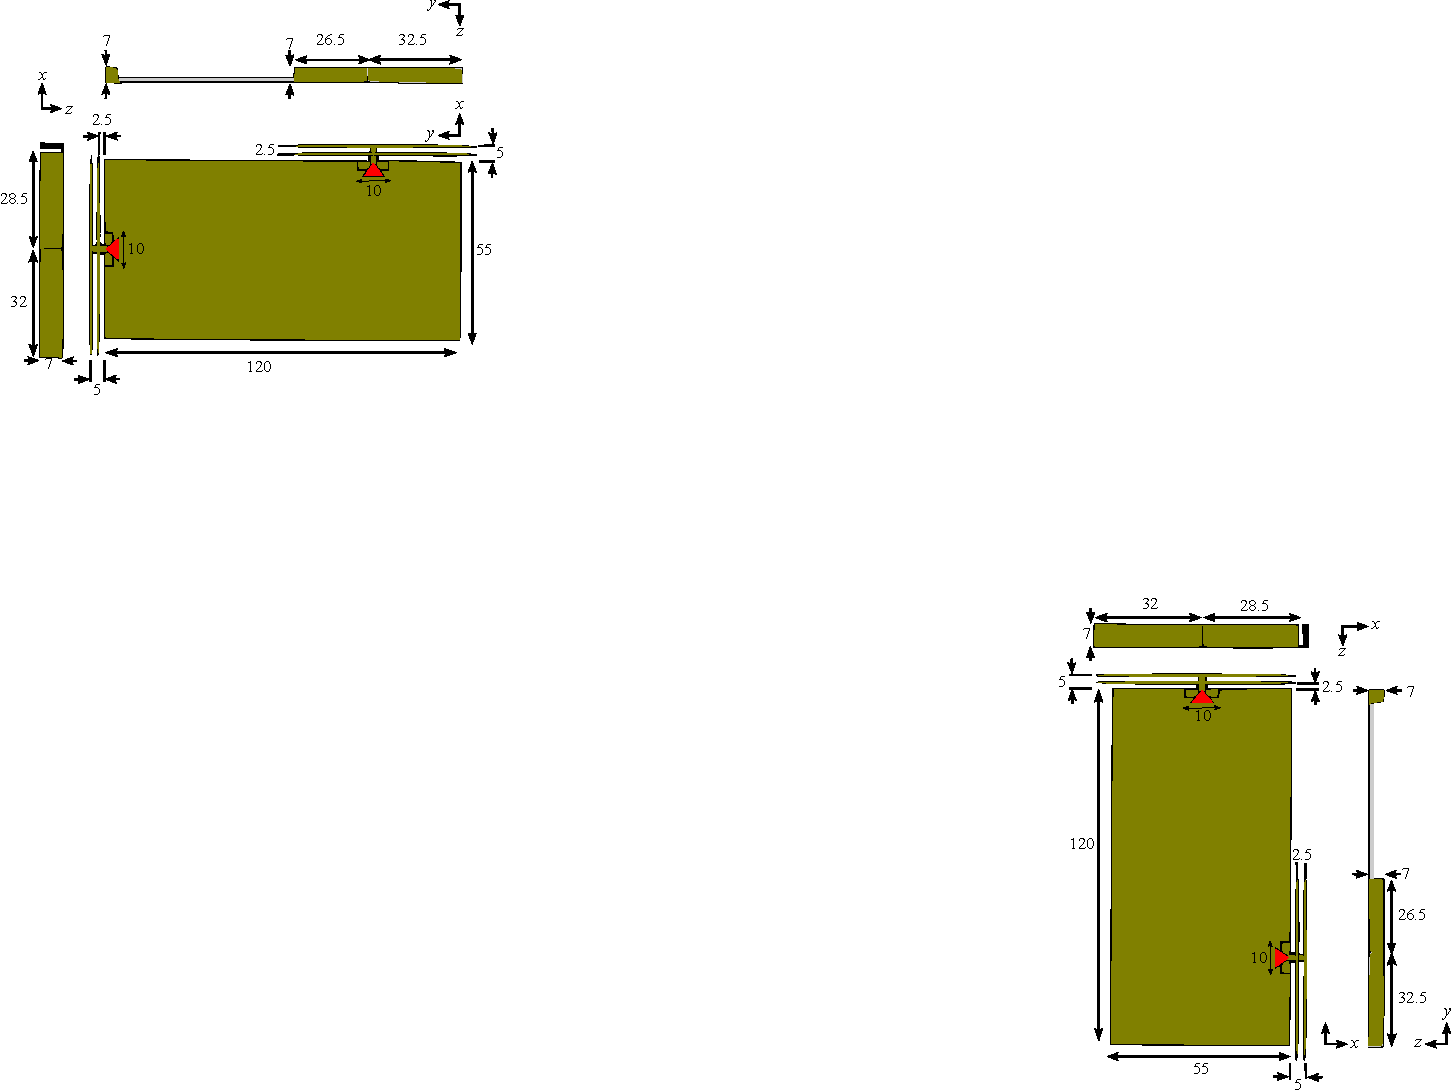
\includegraphics{img/3d_drawing}
  \end{center}
  \caption{Geometry of the MIMO antenna system.}
  \label{fig:antdesign}
\end{figure}


\section{Simulations}
\label{sec:simulations}
The following simulations of the dual-arm non-resonant antenna design are done in CST Microwave Studio using its time-domain solver FIT (Finite Integral Technique). All matching components used are ideal and the simulations are carried out on a bare-board, thus the traces from the tunable MEMS capacitor and SMA connectors are not included in the simulation. 
The antennas, in simplified simulations, are designed to resonate higher than desired as practice has shown detuning when moved to the PCB with MEMS tuners.
The simulations include $S$-parameters, correlation, efficiency in free-space, talk-mode, data-mode, and two-hand-mode. In addition, the peak specific absorption rate (SAR) values of the antenna structures besides a SAM (Specific Antropomorphic Mannequin) head phantom is simulated. The following plots are when sweeping the tuner from around \SI{0.6}{pF} to \SI{6}{pF} (top antenna) and from around \SI{1.2}{pF} to \SI{12}{pF} (side antenna).


%Free space S11 + S22 + Isolation i text
The simulated $S$-parameters are shown in Fig~\ref{fig:sim_sparams}, both antennas cover the low band at \SI{6}{dB} return loss. The high band is however not entirely covered, the top antenna covers from \SIrange{1760}{2550}{MHz} and the side antenna from \SIrange{1710}{2550}{MHz}. The isolation is a minimum of \SI{6}{dB} in the low band and generally higher for the high band with an isolation above \SI{13}{dB}. 
\begin{figure}[tb]
    \centering
    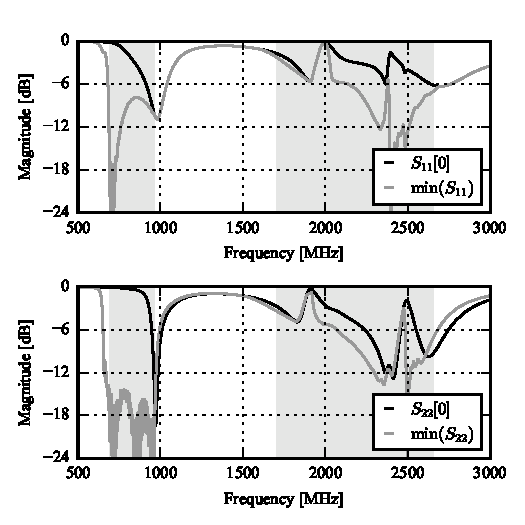
\includegraphics{img/sim/sparams/sparams}
    \caption{Simulated $S$-parameters. Here, $[0]$ marks the minimum capacitance and $\min()$ marks the sweep.}
    \label{fig:sim_sparams}
\end{figure}


%Free space correlation
The correlation simulation is shown in Fig~\ref{fig:sim_corr}, and is sufficiently low for the high band, however the antennas are very correlated in the low band. This is however decreased when simulated with a user. 
\begin{figure}[tb]
    \centering
    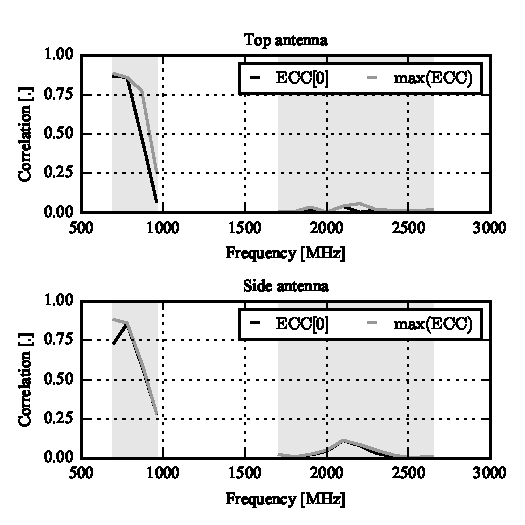
\includegraphics{img/sim/corr/correlation}
    \caption{Simulated envelope correlation coefficient. Here, $[0]$ marks the minimum capacitance and $\max()$ marks the sweep.}
    \label{fig:sim_corr}
\end{figure}


%Free space eff
The efficiency simulation is shown in Fig~\ref{fig:sim_eff}. For the top antenna, the low band can almost be covered at a \SI{-3}{dB} efficiency. The high band has a notch in \SIrange{1905}{2089}{MHz} but apart from this, the entire high band can be covered at an acceptable efficiency. The side antenna can be tuned to cover the high end of the low band at an efficiency above
 \SI{-3}{dB} while the lower part only reaches between \SIrange{-9}{-6}{dB}. The high band has a notch from 1825 MHz to 2010 MHz but has a good efficiency outside this band.
\begin{figure}[tb]
    \centering
    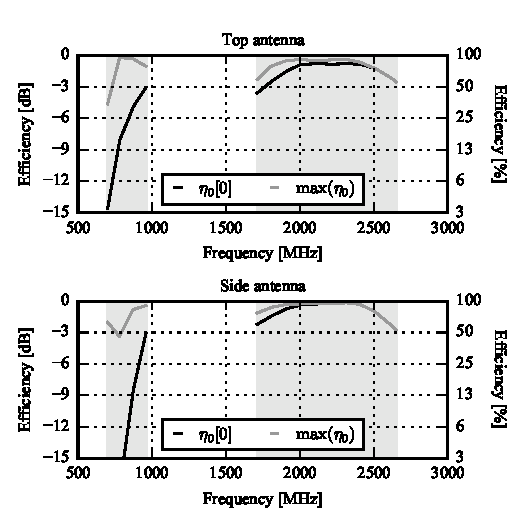
\includegraphics{img/sim/eff/efficiency}
    \caption{Simulated total efficiency. Here, $[0]$ marks the minimum capacitance and $\max()$ marks the sweep. }
    \label{fig:sim_eff}
\end{figure}

%User effects i tabel -> ord 
The user effect simulations showed a general decrease in efficiency and bandwidth and detuned $S$-parameters. The talk-mode simulation shows the worst
detuning and bandwidth coverage compared to the data- and two-hand-mode simulations. But the antennas are still able to cover the desired bandwidth when tuned. Generally the correlation is still quite high in the low band, with a maximum value of 0.8 in the talk-mode case.

%SAR 
The SAR simulation was done at 15 discrete frequencies and with a case and screen. The case is made of BLYAT with a dielectic loss of CYKA\fixme{Shui's materiale???} and the screen is made of perfect electric conductor (PEC) stitched to the ground plane. The simulations showes that both antennas are compliant with the requirement of a maximum SAR of \SI{2}{W/kg}. The top antenna has the highest SAR value of \SI{1.5}{W/kg} in the high band and the side antenna has a maximum SAR value of \SI{0.6}{W/kg} in the high band. 


\section{Measurements}
\label{sec:measurements}

\begin{figure}[tb]
    \centering
    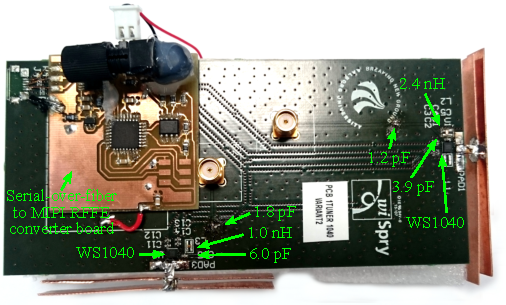
\includegraphics{img/meas/lassedouble}
    \caption{Antenna prototype with MEMS tuners. The converter board converts UART commands from a PC to MIPI RFFE commands, setting the capacitance of the tuners. Component values are annotated.}
    \label{fig:pcb}
\end{figure}

\begin{figure}[tb]
    \centering
    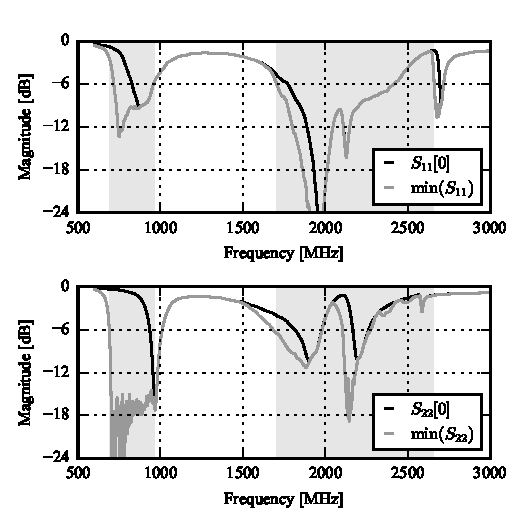
\includegraphics{img/meas/sparams}
    \caption{Measured $S$-parameters for the top and the side antenna when sweeping the tuner from around \SI{0.6}{pF} to \SI{6}{pF} (top antenna) and from around \SI{1.2}{pF} to \SI{12}{pF} (side antenna). Here, $[0]$ marks the minimum capacitance and $\min()$ marks the sweep.}
    \label{fig:meas_sparams}
\end{figure}

The antennas have been built and soldered on to a PCB with a WiSpry WS1040 MEMS tuner for each antenna, as seen in Fig.~\ref{fig:pcb}. Compared to the simplified simulations described in Sec.~\ref{sec:simulations}, the matching at high frequencies appeared troublesome. A shunt capacitor has been soldered onto the transmission lines for each antennas to improve this problem. 
The resulting $S$-parameters are shown in Fig.~\ref{fig:meas_sparams}. It is clear that both antennas cover the low band at \SI{6}{dB} return loss over the tunable range. At the same time, the top antenna covers most of the top band up until \SI{2400}{MHz} while the side antenna lacks bandwidth between \SI{1980}{MHz} and \SI{2110}{MHz} and between \SI{2270}{MHz} and \SI{2650}{MHz}. The isolation loss, $\text{IL}=-|S_{21}|_{\text{dB}}$, is above \SI{12}{dB} at all frequencies, being \SI{12}{dB} at \SI{1870}{MHz}.

\begin{figure}[tb]
    \centering
    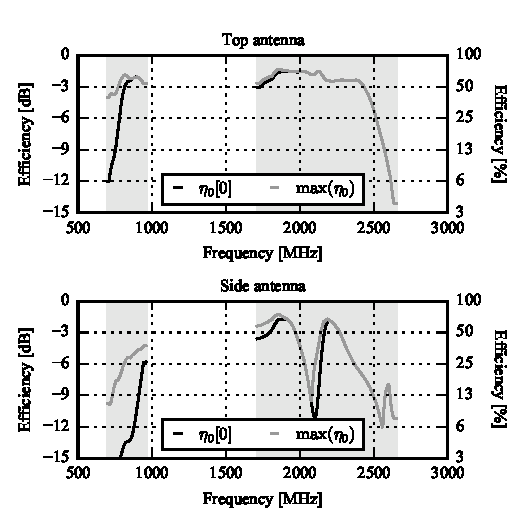
\includegraphics{img/meas/efficiency}
    \caption{Measured total efficiency for the top and the side antenna when sweeping the tuner from around \SI{0.6}{pF} to \SI{6}{pF} (top antenna) and from around \SI{1.2}{pF} to \SI{12}{pF} (side antenna). Here, $[0]$ marks the minimum capacitance and $\max()$ marks the sweep.}
    \label{fig:meas_eff}
\end{figure}

The measured total efficiency when sweeping the tuner is shown in Fig.~\ref{fig:meas_eff}. The top antenna covers all of the low band at around \SI{-3}{dB} efficiency while covering the high band up until \SI{2440}{MHz}. The total efficiency of the side antenna peaks at \SI{-4.1}{dB} in the low band with a minimum at \SI{-9.9}{dB}. The high band is covered from \SI{1710}{MHz} to \SI{1925}{MHz} and from \SI{2095}{MHz} to \SI{2230}{MHz} over its tunable range.


\chapter{Conclusion}
\label{cha:conclusion}
This report has documented the development of digitally tunable LTE antennas supporting MIMO. 

%% Preliminary designs
Three preliminary designs, which all cover the required bands in free space, have been designed. Each designs has its strengths and weaknesses and they all use a ground clearance of \SI{9.5}{mm} to \SI{10}{mm} for the top antenna and \SI{7}{mm} to \SI{9.5}{mm} for the side antenna. 

The three preliminary designs were also simulated, in the proximity of a user, in data mode, play mode, and talk mode. Here, the triangle-feed designs as well as the dual-feed design generally held up the best although severe detuning was apparent in every design. The Specific Absorption Rate (SAR) was also simulated and every design met the requirements of a maximum SAR of \SI{2}{W/kg}.

The simulations were simplified, not taking into account non-ideal components, component placement, and transmission lines. To get a more accurate picture of the performance, prototypes were built of the three preliminary designs. The $S$-parameters and the total efficiency were measured for a variety of discrete tuning capacitor values. The folded monopole design did not cover the low band very well and the dual-feed design was not tunable in the side antenna. For this reason, the triangle-feed design was chosen as the first design to be realized on a PCB with a MEMS tuner.

%% The effect of ground clearance -> 5mm minimized design
As the space for antennas in today's mobile phones is limited by the large screen size, a smaller design was developed to also be implemented with the tuner PCB. An investigation of the effect of lowering the ground clearance was made, and showed that a very reasonable tunable design could be realized with only \SI{5}{mm} of ground clearance -- on a par with the preliminary designs over the tunable range. The minimized design was measured with the tuner PCB but showed problems covering the high band. The design was therefore modified with an extra pair of arms before the final implementation with the tuner PCB.

The triangle-feed design, like the minimized design, showed problems covering the high end of the high band when moved to the tuner PCB. The low band, for both the top and the side antenna, as well as most of the high band for the top antenna was covered acceptably, while the side antenna was not resonating as required in the high band.

The modified minimized design, while being slightly better in the high band, still had trouble in the very high end of the spectrum. For the final design, it was observed that adding a small amount of shunt capacitance near the middle of the transmission lines, going from the SMA connectors to the antennas, improved the high-band performance vastly. The resulting design showed that the top antenna was able to cover the whole low band at above \SI{-4}{dB} total efficiency and the high band above \SI{-3}{dB} from \SI{1710}{MHz} to around \SI{2500}{MHz}. From \SI{2500}{MHz} and up, the efficiency decreased. The side antenna generally showed a lower bandwidth and efficiency with a total efficiency from \SI{-10}{dB} to \SI{-4.5}{dB} in the low band and an efficiency above \SI{-3}{dB} from around \SI{1710}{MHz} to around \SI{2300}{MHz} except for a notch around \SI{2000}{MHz}. These results show that a low-ground clearance design is possible while still covering most of the LTE bands at an acceptable total efficiency.

%% Correlation high -> only MIMO above x MHz
The envelope correlation has been simulated for all designs. In order to have good MIMO performance, a low correlation -- below 0.5 -- is desired. The modified minimized design showed a correlation above 0.5 from \SI{700}{MHz} to around \SI{900}{MHz} in free space which makes it unsuited for MIMO applications in the low band. The correlation is much lower in the high band, so MIMO could still be used at these frequencies. In the user effect simulations, the correlation in the low band generally dropped, making the MIMO useful in part of the low band as well. The high correlation at low frequencies is to be expected as a large part of the ground plane is used as a radiating element for both top and side antenna, making the radiation patterns more similar. MIMO and diversity schemes would therefore be better implemented at higher frequencies.

\newpage

%% Comparison with state-of-the-art
% vim:nowrap

\def\MARK{$^{\dagger}$\xspace}
\begin{table}[htbp]
    \centering
    \footnotesize
    \begin{tabularx}{\linewidth}{p{24mm}Xk{13mm}k{17mm}k{13mm}k{20mm}k{17mm}k{17mm}}
        \toprule
        &&&&&& \multicolumn{2}{c}{$\eta_{\text{tot}}$ of main antenna} \\\cline{7-8}
        Antenna & Note & Tuner type & Antenna volume (\si{mm\cubed}) & Antenna area (\si{mm\squared}) & Total dimensions (\si{mm\cubed}) & Low band (\si{\%}) & High band (\si{\%})  \\
        \midrule
        Monopole top                         & Monopole                    & Discrete & 3885   & 555   & $130\times62\times7$     & 38--60 & 43--98        \\
        Monopole side                        & Monopole                    & Discrete & 2646   & 378   & $130\times62\times7$     & 28--64 & 31--84        \\
        \midrule
        Triangle-feed top                    & Non-resonant and microstrip & Discrete & 4340   & 620   & $140\times69\times7$     & 47--70 & 59--92        \\
        Triangle-feed top                    & Non-resonant and microstrip & MEMS     & 4340   & 620   & $140\times69\times7$     & 46--71 & 13--67        \\
        Triangle-feed side                   & Non-resonant and microstrip & Discrete & 4550   & 650   & $140\times69\times7$     & 48--72 & 59--91        \\
        Triangle-feed side                   & Non-resonant and microstrip & MEMS     & 4550   & 650   & $140\times69\times7$     & 29--51 & $<3$--49\MARK \\
        \midrule
        Non-resonant top                     & Non-resonant                & Discrete & 2850   & 570   & $129.5\times67\times6.6$ & 61--94 & 23--86        \\
        Non-resonant side                    & Non-resonant                & Discrete & 3087.5 & 617.5 & $129.5\times67\times6.6$ & 5--43  & 62--88        \\
        \midrule
        Mod.\ minimized top               & Double-monopole             & MEMS     & 2117.5 & 302.5 & $130\times62\times7$     & 43--65 & 4--72\MARK    \\
        Mod.\ minimized side              & Double-monopole             & MEMS     & 2065   & 295   & $130\times62\times7$     & 10--37 & 7--73\MARK    \\
        \midrule
        \cite{ilvonen2014multiband} main     & Planar ProtoM               & MEMS     & 1170   & 900   & $120\times60\times1.5$   & 30--57 & 44–78         \\
        \cite{ilvonen2014multiband} aux      & Planar ProtoM               & MEMS     & 1170   & 900   & $120\times60\times1.5$   & 29--57 & 43--78        \\
        \cite{ilvonen2014multiband} main     & ProtoM                      & MEMS     & 3900   & 900   & $120\times60\times5$     & 49--72 & 56--88        \\
        \cite{ilvonen2014multiband} aux      & ProtoM                      & MEMS     & 3900   & 900   & $120\times60\times5$     & 48--72 & 55--88        \\
        \cite{morris2014tunable}             & Monopole                    & MEMS     & 1500   & ?     & ?                        & 28--60 & 45--97        \\
        \cite{xia2015compact}                & IFA                         & CMOS     & 1620   & 270   & $110\times45\times6$     & 54--65 & 70--?         \\
        \cite{tatomirescu2015alternative} RX & Monopoles, not tuned        & MEMS     & 300    & 300   & $120\times55\times1$     & 50--?  & --            \\
        \cite{tatomirescu2015alternative} TX & Folded IFA, tuned           & MEMS     & 640    & 160   & $120\times55\times?$     & 32--59 & --            \\
        \cite{trinh2016reconfigurable}       & Monopole                    & CMOS     & 2400   & 400   & $130\times70\times6.8$   & 40--63 & 20--85        \\
        \bottomrule
    \end{tabularx}
    \caption{Comparison of reconfigurable LTE antenna designs (measured free space parameters). The total efficiencies the maximum obtainable bandwidth in-band for all measured capacitor values. \MARK{}Not all of the bands are covered -- this is the very-worst case measured in the specified band although most of the band may be covered.}
    \label{tab:comparison_reconf_lte}
\end{table}

% morris2014tunable Tunable Antennas for Mobile Devices: Achieving High Performance in Compelling Form Factors 
% http://ieeexplore.ieee.org/stamp/stamp.jsp?tp=&arnumber=6848618
% - No size given
% 
% A Compact Multi-band Tunable LTE Antenna for Mobile Applications
% http://ieeexplore.ieee.org/stamp/stamp.jsp?tp=&arnumber=7304964
% - Low sample size
% 
% Alternative Duplexing for LTE FDD using the Theory of Characteristic Modes
% http://ieeexplore.ieee.org/stamp/stamp.jsp?tp=&arnumber=7228959
% - Low sample size, only low band
% 
% Reconfigurable Antenna for Future Spectrum Reallocations in 5G Communications
% http://ieeexplore.ieee.org/stamp/stamp.jsp?tp=&arnumber=7347359


All the measured designs from from the report are summarized in Table~\ref{tab:comparison_reconf_lte} together with the designs discussed in the introduction, Chapter~\ref{cha:intro}. Here, the range of total efficiency for each design is shown, for both the low and the high band, as well as the dimensions of the designs. 

In the low band, most of the measurements show comparable efficiencies to the state-of-the-art designs. In the high band, the prototypes on copper clad board with discrete components also show very comparable results. It is clear that the efficiency in the high band is severely lower on the tuner PCB. The small minimum value is due to some part of the high band not being covered while most of the band \emph{is} covered at above \SI{-3}{dB}.

The top antenna of the modified minimized design, with only \SI{5}{mm} ground clearance, is very much on a par with designs with much more ground clearance (up to \SI{2500}{MHz}) while the side antenna suffers from a few in-band notches. 

Compared to \cite{ilvonen2014multiband}, the area is smaller due to the low ground clearance, while the volume of the antenna is larger as the height is \SI{7}{mm}. A natural next step would be to try to lower the height to make the design even more compact, as done in \cite{ilvonen2014multiband}. Another next step would be to re-design the PCB to see if the high-band performance can be improved. In this case, the RFFE optical interface could be incorporated into the board as well.

A \SI{5}{mm} version of the triangle-feed design may be successful if capacitance is added to the transmission line as with the modified minimized design. The \SI{10}{mm} version appeared to be well-behaved so this design might also be good for LTE if it could be minimized.

The results show that it is possible to design LTE antennas with only \SI{5}{mm} ground clearance while still having an acceptable total efficiency over the range of the tuner.


%%%%%%%%%%bib%%%%%%%%%%%%
\bibliographystyle{ieeetr}
\bibliography{bib/sources}

\end{document}
